\documentclass[conference]{IEEEtran}
\usepackage{booktabs}
\usepackage{graphicx}
\usepackage{url}
\usepackage{balance}

\graphicspath{{../results/charts/}}
\newcommand{\project}{\mbox{PSYCON}}

\title{\project: A Multimodal Wearable System for Psychological State Detection}

\author{
  \IEEEauthorblockN{Arjun Vijay Prakash}
  \IEEEauthorblockA{
    Software and Machine Learning\\
    Grade 11 Student\\
    City Montessori School, Quality Building\\
    Sector G, LDA Colony, Kanpur Road\\
    Lucknow, Uttar Pradesh 226012, India
  }
  \and
  \IEEEauthorblockN{Saksham Yadav}
  \IEEEauthorblockA{
    Hardware and Wearable System\\
    Grade 11 Student\\
    City Montessori School, Quality Building\\
    Sector G, LDA Colony, Kanpur Road\\
    Lucknow, Uttar Pradesh 226012, India
  }
}

\begin{document}

\maketitle

\begin{abstract}
This paper presents \project, the Psychophysiological Condition Observation Network, a prototype multimodal wearable system for estimating psychological state from physiological, motion, and audio-derived signals. The current software pipeline is validated using the public WESAD dataset before adaptation to \project{} hardware data, pending IRB guidance. The implemented pipeline extracts ten-second feature windows from wearable signals and compares rule-based, logistic regression, random forest, XGBoost, and LightGBM classifiers across single-modality and multimodal feature sets. The pipeline also adds per-subject baseline-difference features to support the project's personalization goal.
\end{abstract}

\section{Introduction}

Stress detection using wearable sensors is challenging because individual signals can be noisy and ambiguous. Heart and electrodermal signals can change due to stress, but also due to temperature, activity, sensor contact, or individual physiology. Motion can indicate agitation, but it can also indicate ordinary movement. \project{} explores whether multimodal sensing can improve robustness compared with single-modality approaches.

The long-term system consists of a wrist biosensing module, an ear/audio module, and a mobile application for synchronization, inference, visualization, and storage. The present work focuses on the software and machine learning foundation. It uses WESAD, a public multimodal wearable stress and affect dataset, to validate the pipeline before collecting human-participant data from \project{} hardware \cite{schmidt2018wesad}.

The central product idea is personalization. Instead of using raw physiological values directly, \project{} should establish a calm baseline for each user during first wear and predict stress from deviations from that baseline.

\section{Methods}

The current implementation validates the software and modeling pipeline using WESAD pickle files as the source of truth, because they contain aligned physiological signals and labels. The pipeline is reproducible from the repository root with \texttt{python main.py}. Raw WESAD data is stored locally and excluded from version control.

Wrist signals are mapped to \project{} concepts as follows: WESAD EDA is treated as a GSR proxy, accelerometer data is treated as motion, BVP is treated as a heart-signal proxy, and temperature is retained as an optional contextual feature. Signals are resampled to a common 4 Hz timeline. Ten-second windows with a two-second hop are used for feature extraction.

The first classifier is binary: WESAD baseline is mapped to calm and WESAD stress is mapped to high stress. Amusement and other labels are ignored for the first model. Mild stress remains reserved for future \project-specific participant data because WESAD does not provide a direct mild-stress class.

Extracted features include EDA mean, standard deviation, range, slope, and peak count; BVP mean, standard deviation, range, slope, and peak count; accelerometer magnitude and jerk features; and temperature mean, standard deviation, range, and change. Per-subject calm baselines are computed from WESAD baseline windows, and baseline-difference features are added before model training. The evaluation compares rule-based, logistic regression, random forest, XGBoost, and LightGBM models across single-modality and multimodal feature sets.

The train-test split is grouped by subject so that windows from held-out subjects are used for evaluation. This is stricter than a random window-level split and better reflects generalization to unseen users.

\section{Results}

The current WESAD run produced 13,698 labeled windows from 15 subjects after filtering to calm and high-stress periods. The dataset contained 8,760 calm windows and 4,938 high-stress windows. Table~\ref{tab:model-results} reports the top results from the latest reproducible pipeline run.

\begin{table}[h]
\centering
\caption{Top WESAD Model Results}
\label{tab:model-results}
\begin{tabular}{llrrrr}
\toprule
Model & Modality & Acc. & Prec. & Rec. & FPR \\
\midrule
XGBoost & EDA only & 0.932 & 0.871 & 0.953 & 0.081 \\
LightGBM & EDA only & 0.924 & 0.871 & 0.928 & 0.078 \\
Logistic regression & EDA only & 0.917 & 0.827 & 0.977 & 0.117 \\
Logistic regression & Multimodal & 0.915 & 0.814 & 0.995 & 0.130 \\
Random forest & Multimodal & 0.869 & 0.865 & 0.758 & 0.067 \\
XGBoost & Multimodal & 0.864 & 0.877 & 0.727 & 0.058 \\
\bottomrule
\end{tabular}
\end{table}

The strongest current result was obtained by an EDA-only XGBoost model, followed by EDA-only LightGBM and EDA-only logistic regression. The best multimodal model was logistic regression, which remained close to the top single-modality results and achieved the highest recall among the top models. This result is scientifically useful: WESAD appears to be strongly driven by electrodermal activity, while \project's hardware data still needs to test whether motion, audio features, and per-user baselines reduce false positives in real-world conditions.

\begin{figure}[h]
\centering
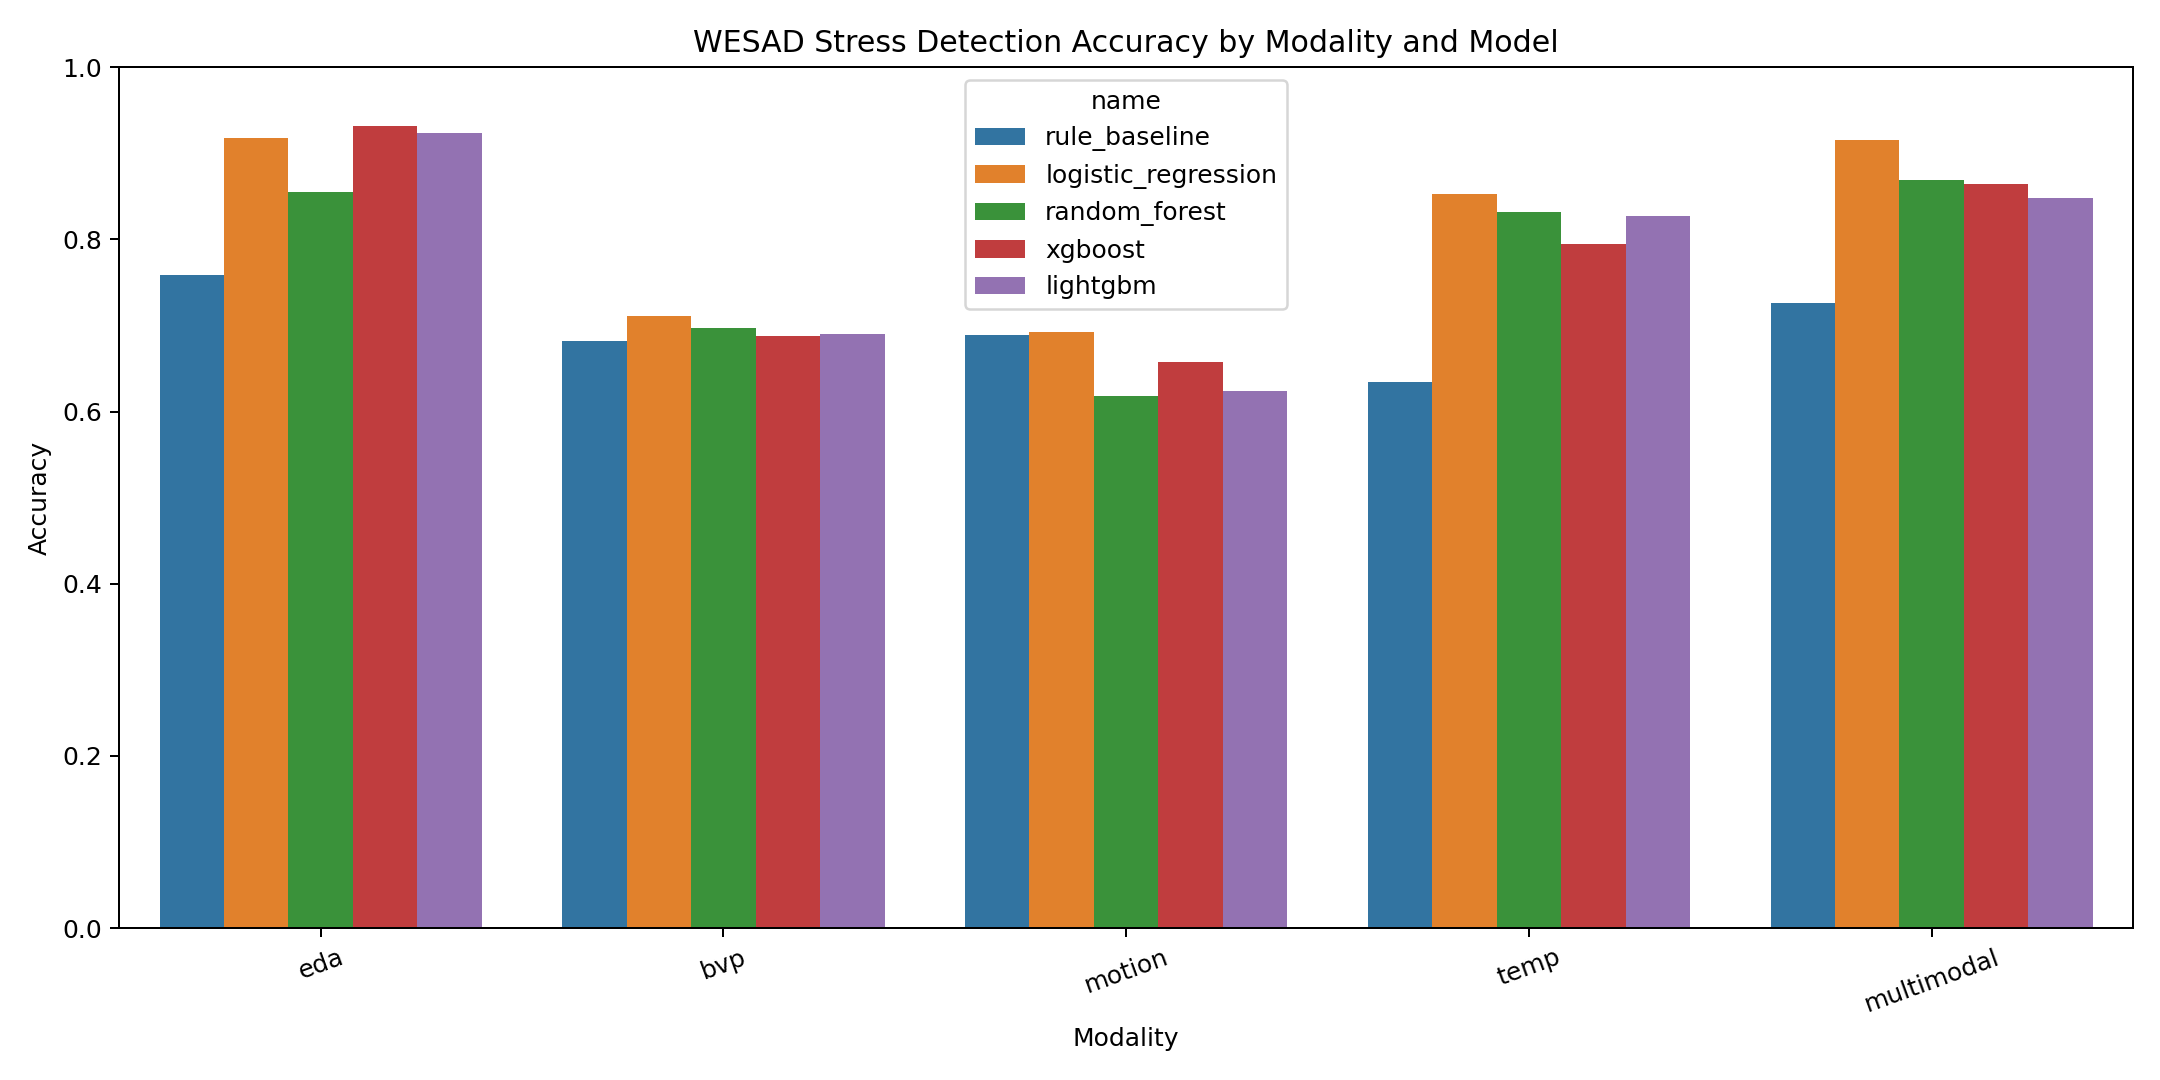
\includegraphics[width=0.95\linewidth]{model_comparison.png}
\caption{Accuracy comparison across model families and signal modalities.}
\label{fig:model-comparison}
\end{figure}

\section{Discussion}

The WESAD results validate the software and machine learning approach, but they do not prove accuracy on \project{} hardware. WESAD uses different sensors and does not include the planned trigger-based audio feature stream. Therefore, the current result should be framed as software-pipeline validation rather than device validation.

The results also show why machine learning is useful in this project. Rule-based thresholds provide an interpretable baseline, but learned models improve performance by combining weak signals into a stronger prediction. The best models used multiple modalities, which aligns with the project hypothesis. Future \project{} hardware data should extend this approach by using each user's first-wear baseline rather than only a generic population model.

There are several limitations. The first classifier is binary because WESAD does not provide a direct mild-stress class. The model therefore maps scores to calm, mild stress, and high stress for output, but true mild-stress training requires future \project-specific labeled data. Human participant collection must wait for IRB guidance or approval. Audio privacy also remains important; the MVP should prefer audio features over continuous raw audio.

Future work will adapt the pipeline to \project{} hardware data, add participant-specific baseline calibration, evaluate trigger-based audio features, and compare the deployed on-device inference result with offline research models.

\balance
\bibliographystyle{IEEEtran}
\bibliography{references}

\end{document}
